\documentclass[10pt,a4paper]{article}

\usepackage{iftex}
\ifPDFTeX
  \usepackage[T1]{fontenc}
  \usepackage[utf8]{inputenc}
\fi
\usepackage[brazil]{babel}
\usepackage{newtxtext,newtxmath}
\usepackage[a4paper,top=1.8cm,bottom=1.8cm,left=2cm,right=2cm]{geometry}
\usepackage{graphicx}
\usepackage{booktabs}
\usepackage{amsmath}
\usepackage{xcolor}
\usepackage[font=small,labelfont=bf,skip=3pt]{caption}
\usepackage{enumitem}
\usepackage{titlesec}
\usepackage[hidelinks]{hyperref}

\setlist{nosep,leftmargin=*}
\titleformat*{\section}{\large\bfseries}
\titleformat*{\subsection}{\normalsize\bfseries}
\titlespacing*{\section}{0pt}{7pt}{3pt}
\titlespacing*{\subsection}{0pt}{5pt}{2pt}
\setlength{\parskip}{2pt}
\setlength{\textfloatsep}{8pt}

% Pendências a completar antes da entrega (aparecem em vermelho no PDF)
\newcommand{\pendente}[1]{\textcolor{red}{#1}}
\newcommand{\term}[1]{\textit{#1}}      % termo, token ou trecho em inglês
\newcommand{\rel}[1]{\textbf{#1}}       % documento relevante
\newcommand{\fonte}[1]{#1$^\dagger$}    % documento-fonte (julgamento -1)

\begin{document}

\begin{center}
  {\Large\bfseries Modelo Vetorial vs.\ BM25 na coleção Cranfield:\\[2pt]
  pré-processamento, parâmetros e análise de erros}\\[6pt]
  Ana Paula de Abreu Batista (nº USP 12688424)\\
  Instituto de Ciências Matemáticas e de Computação (ICMC), Universidade de São Paulo (USP), São Carlos -- SP\\
  \pendente{[e-mail]}\\[3pt]
  {\small SCC0282 -- Recuperação de Informação -- Trabalho Prático 1 -- 2º semestre de 2026}
\end{center}

\section{Introdução}

Sistemas de recuperação de informação ordenam documentos pela relevância estimada para a necessidade expressa em uma consulta. Os modelos clássicos de casamento de termos, o Modelo Vetorial e o modelo probabilístico BM25, continuam sendo referências importantes, e entender por que eles acertam ou erram em cada consulta ajuda a interpretar seu comportamento~\cite{manning}. Este trabalho implementa os dois modelos sobre a coleção Cranfield e os compara quantitativa e qualitativamente. Os objetivos são: medir o efeito do pré-processamento; comparar os modelos consulta a consulta; avaliar a sensibilidade do BM25 aos parâmetros $k_1$ e $b$; testar reformulações de consultas; e investigar erros. Os resultados são relacionados a conceitos como frequência de termos, saturação, normalização por comprimento e descompasso vocabular. O código está no notebook \texttt{trabalho\_pratico\_recinfo.ipynb}, e os resultados por consulta, na pasta \texttt{resultados/}.

\section{Técnicas Utilizadas}

\subsection{Pré-processamento}
Os textos são convertidos para minúsculas e tokenizados com a expressão regular \verb|\w+| (\texttt{RegexpTokenizer} do NLTK), que descarta a pontuação e separa palavras compostas (\term{three-dimensional} $\to$ \term{three}, \term{dimensional}). Sobre os tokens, aplicamos opcionalmente a remoção de stopwords (lista em inglês do NLTK) e o stemming de Porter~\cite{porter}. Isso gera quatro configurações: \texttt{basico} (nenhum dos dois), \texttt{stopwords}, \texttt{stemming} e \texttt{both} (ambos). O mesmo pré-processamento é aplicado a documentos e consultas. Os documentos são indexados como título + texto. Como o campo de texto do Cranfield já começa repetindo o título (1.398 dos 1.400 documentos), isso na prática duplica o título e dá mais peso aos seus termos. A Seção~\ref{sec:preproc} mostra que essa escolha melhora os dois modelos.

\subsection{Modelo Vetorial}
Documentos e consultas são vetores no espaço do vocabulário, com pesos TF-IDF calculados pelo \texttt{TfidfVectorizer} do scikit-learn~\cite{sklearn}, com os parâmetros explícitos \texttt{smooth\_idf=True}, \texttt{sublinear\_tf=False} e \texttt{norm='l2'}:
\[
  w_{t,d} = tf_{t,d}\cdot idf_t,\qquad idf_t = \ln\frac{1+N}{1+df_t} + 1,\qquad
  \mathrm{sim}(q,d)=\frac{\vec q\cdot\vec d}{\lVert\vec q\rVert\,\lVert\vec d\rVert}=\sum_t \hat q_t\,\hat d_t ,
\]
onde $tf_{t,d}$ é a contagem bruta do termo, $N=1400$ e $df_t$ é o número de documentos que contêm o termo. O vocabulário e o IDF são aprendidos só nos documentos, e a consulta é projetada no mesmo espaço (\texttt{transform}). Como o $tf$ não é saturado, o peso cresce linearmente com a repetição. Já a normalização L2 faz o score depender do quanto os termos da consulta dominam o vetor do documento, e não do tamanho absoluto dele. Pelo ``$+1$'' fora do logaritmo, até um termo presente em todos os documentos tem $idf=1$.

\subsection{Modelo probabilístico BM25}
O BM25~\cite{robertson} foi implementado manualmente na classe \texttt{BM25Modelo}, sem bibliotecas de ranking. O construtor pré-calcula a frequência de cada termo em cada documento, o comprimento $|d|$ de cada documento, a média $avgdl$ e o IDF de cada termo. O score é
\[
  \mathrm{score}(q,d)=\sum_{t\in q} IDF(t)\,\frac{f_{t,d}\,(k_1+1)}{f_{t,d}+k_1\!\left(1-b+b\,\frac{|d|}{avgdl}\right)},\qquad
  IDF(t)=\ln\!\left(\frac{N-df_t+0{,}5}{df_t+0{,}5}+1\right).
\]
O IDF com ``$+1$'' (variante do Lucene) nunca é negativo. $k_1$ controla a saturação da frequência do termo no documento (com $k_1\to0$ o modelo fica binário), e $b$ controla a normalização pelo comprimento ($b=0$: nenhuma; $b=1$: total). A soma percorre os tokens da consulta com repetição, então um termo repetido na consulta conta em dobro, e não há saturação da frequência na consulta (parâmetro $k_3$). Na comparação principal usamos $k_1=1{,}5$ e $b=0{,}75$, valores usuais na literatura. Nos dois modelos, documentos com score zero ficam fora do ranking.

\section{Avaliação}

Usamos a coleção Cranfield, obtida com a biblioteca \texttt{ir\_datasets}~\cite{irds}, que baixa o arquivo original da Universidade de Glasgow: 1.400 resumos de artigos de aeronáutica, 225 consultas e 1.837 julgamentos, os mesmos em todos os experimentos. Os graus dos julgamentos se distribuem em $-1$ (225), 1 (128), 2 (387), 3 (734) e 4 (363). Na escala de Cleverdon~\cite{cleverdon}, registrada no arquivo \texttt{cranqrel.readme} da coleção, 1 significa ``resposta completa'' e 4, ``interesse mínimo''. A documentação do \texttt{ir\_datasets} descreve a ordem inversa, mas a biblioteca repassa os valores originais sem transformá-los, e por isso seguimos o readme.

\textbf{Relevância.} Para P@10, R@10, F1@10, MAP e MRR, é relevante todo documento com grau $\geq1$, e julgamentos $-1$ e documentos não julgados são não relevantes. Todas as 225 consultas têm ao menos um relevante. No NDCG@10 usamos relevância graduada com ganho $g=5-\text{grau}$ (grau 1 $\to$ ganho 4), respeitando a escala original. Há exatamente um julgamento $-1$ por consulta, em geral um documento muito próximo dela: no BM25, ele está no Top 10 em 72\% das consultas, e o da consulta 1, por exemplo, é \term{similarity laws for aerothermoelastic testing}. O padrão é consistente com a metodologia do Cranfield~II, em que autores formularam perguntas a partir dos próprios artigos~\cite{cleverdon}. Tudo indica que o documento $-1$ é o \emph{artigo-fonte} da pergunta. Seguimos a especificação e o tratamos como não relevante, mas o destacamos na análise (marcado com $\dagger$).

\textbf{Métricas.} P@10 e R@10; F1@10 (média harmônica das duas); AP calculada sobre o ranking completo e dividida pelo total de relevantes da consulta, com o MAP como sua média; MRR; e NDCG@10. Todas são guardadas por consulta (CSVs em \texttt{resultados/}) e agregadas pela média sobre as 225 consultas.

\textbf{Configurações.} (i) 4 pré-processamentos $\times$ 2 modelos (BM25 com $k_1=1{,}5$, $b=0{,}75$); (ii) comparação por consulta e análise de casos com \texttt{both}; (iii) grade $k_1\in\{0{,}5;\,1{,}2;\,2{,}0\}\times b\in\{0;\,0{,}75;\,1\}$ com \texttt{both}, comparada por MAP, P@10 e NDCG@10; (iv) modificação de consultas e análise de erros com \texttt{both} e a melhor combinação da grade ($k_1=2{,}0$, $b=0{,}75$). Os qrels são usados só para avaliar, nunca para alterar rankings. Como o melhor pré-processamento e os melhores parâmetros são escolhidos pelo MAP nas mesmas consultas avaliadas, os números da etapa (iv) são levemente otimistas.

\section{Resultados Obtidos e Análise}

\begin{table}[!htb]
  \centering\small
  \caption{Métricas médias nas 225 consultas, por pré-processamento e modelo (BM25 com $k_1=1{,}5$, $b=0{,}75$).}
  \label{tab:geral}
  \begin{tabular}{llcccccc}
    \toprule
    Pré-processamento & Modelo & P@10 & R@10 & F1@10 & MAP & MRR & NDCG@10\\
    \midrule
    \texttt{basico}    & Vetorial & 0,227 & 0,371 & 0,254 & 0,278 & 0,505 & 0,341\\
                       & BM25     & 0,230 & 0,388 & 0,261 & 0,282 & 0,506 & 0,349\\
    \texttt{stopwords} & Vetorial & 0,224 & 0,370 & 0,252 & 0,284 & 0,516 & 0,341\\
                       & BM25     & 0,237 & 0,401 & 0,270 & 0,296 & 0,529 & 0,366\\
    \texttt{stemming}  & Vetorial & 0,234 & 0,385 & 0,262 & 0,298 & 0,516 & 0,355\\
                       & BM25     & 0,237 & 0,397 & 0,268 & 0,307 & 0,535 & 0,371\\
    \texttt{both}      & Vetorial & \textbf{0,243} & 0,402 & 0,273 & 0,307 & 0,534 & 0,367\\
                       & BM25     & \textbf{0,243} & \textbf{0,407} & \textbf{0,275} & \textbf{0,319} & \textbf{0,551} & \textbf{0,380}\\
    \bottomrule
  \end{tabular}
\end{table}

\subsection{Pré-processamento}\label{sec:preproc}
A configuração \texttt{both} é a melhor nos dois modelos (Tabela~\ref{tab:geral}). Em relação a \texttt{basico}, o MAP sobe 13\% no BM25 (0,282 $\to$ 0,319) e 11\% no Vetorial (0,278 $\to$ 0,307). O stemming sozinho contribui mais que a remoção de stopwords sozinha: MAP de 0,307 contra 0,296 no BM25, e de 0,298 contra 0,284 no Vetorial. O Porter reduz o vocabulário de 7.471 para 4.820 termos, agrupando variantes (\term{heated}/\term{heating} $\to$ \term{heat}), o que aumenta os casamentos entre consulta e documento. Mas ele não agrupa \term{theory}/\term{theoretical} (\term{theori}/\term{theoret}) nem \term{sudden}/\term{suddenly}, falhas que reaparecem na análise de erros. A remoção de stopwords ajuda porque as consultas são perguntas (38,6\% dos seus tokens são stopwords) e algumas stopwords têm IDF alto no corpus: \term{what} ocorre em só 16 resumos (idf 5,41 no TF-IDF) e favorece esses documentos sem motivo. No TF-IDF, o ``$+1$'' do IDF também mantém \term{the} e \term{of} com peso $\approx1$, e essas palavras inflam a norma dos vetores (as stopwords são 41\% dos tokens dos documentos). O ganho não é uniforme: no BM25, \texttt{both} supera \texttt{basico} em 139 consultas e perde em 75. Por fim, indexar só o texto (título 1$\times$) em vez de título + texto (título 2$\times$) reduz o MAP de 0,319 para 0,307 no BM25 e de 0,307 para 0,294 no Vetorial. Dobrar a frequência dos termos do título, que resumem o assunto central, funciona como um reforço de peso.

\subsection{Comparação entre o Modelo Vetorial e o BM25}
Com \texttt{both}, o BM25 é ligeiramente melhor na média (MAP 0,319 contra 0,307; MRR 0,551 contra 0,534; NDCG@10 0,380 contra 0,367), e a P@10 é idêntica (0,243). A média, porém, esconde diferenças grandes nos dois sentidos (Figura~\ref{fig:dap}). O BM25 tem AP maior em 121 consultas, o Vetorial em 96, há 8 empates, e 52 consultas têm $|\Delta AP|>0{,}1$. A Tabela~\ref{tab:casos} mostra os casos extremos pedidos na especificação. A análise a seguir decompõe os scores por termo (função \texttt{decompor\_scores} do notebook); ``Q$n$'' indica a consulta $n$.

\begin{figure}[!htb]
  \centering
  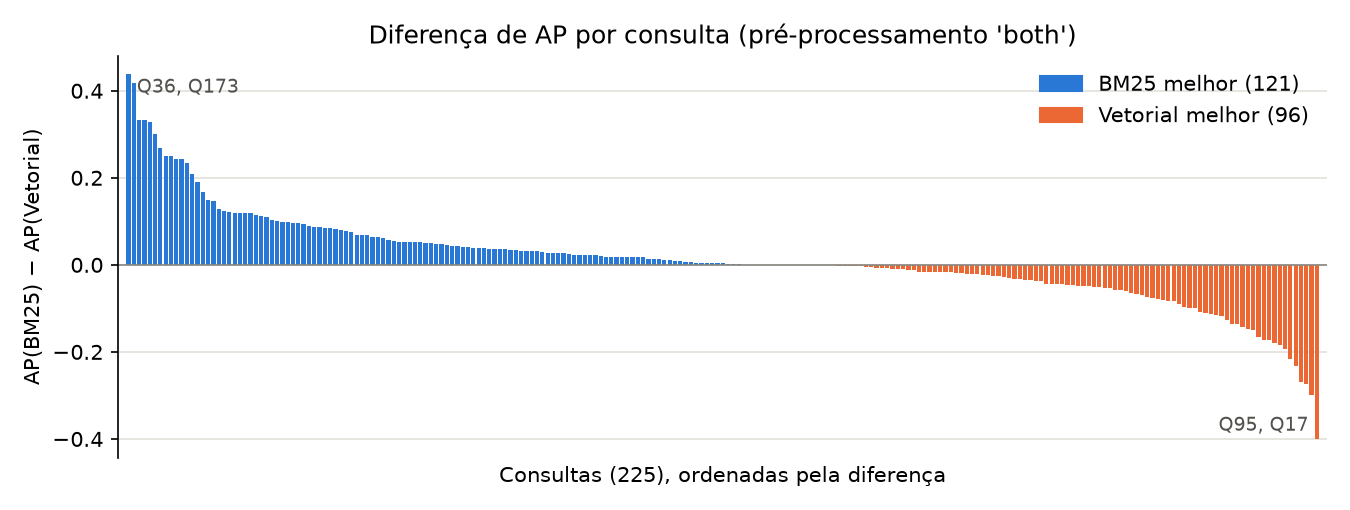
\includegraphics[width=0.82\linewidth]{resultados/grafico_diferenca_ap_por_consulta.png}
  \caption{Diferença de AP (BM25 $-$ Vetorial) por consulta, com pré-processamento \texttt{both}. As consultas das pontas são analisadas na Seção~\ref{sec:casos}.}
  \label{fig:dap}
\end{figure}

\begin{table}[!htb]
  \centering\small
  \caption{Top 5 de cada modelo nos casos analisados (\texttt{both}; BM25 com $k_1=1{,}5$, $b=0{,}75$). Documentos relevantes em \textbf{negrito}; $\dagger$ = documento-fonte (julgamento $-1$).}
  \label{tab:casos}
  \begin{tabular}{llcclll}
    \toprule
    Caso & Q & AP Vet. & AP BM25 & Top 5 Vetorial & Top 5 BM25\\
    \midrule
    BM25 melhor     & 36  & 0,064 & 0,502 & 398, 303, 564, 554, 623 & \rel{168}, 623, 123, \fonte{518}, 550\\
                    & 173 & 0,583 & 1,000 & \fonte{532}, \rel{367}, \rel{451}, 917, 1073 & \rel{367}, \rel{451}, \fonte{532}, 917, 767\\
    Vetorial melhor & 17  & 0,508 & 0,107 & \rel{106}, 1281, 700, 1301, \fonte{498} & 1108, 1281, 700, 336, \rel{106}\\
                    & 95  & 0,750 & 0,450 & \rel{662}, \fonte{635}, 1258, \rel{283}, 1191 & \fonte{635}, \rel{662}, 1002, 553, \rel{283}\\
    Ambos ruins     & 13  & 0,000 & 0,000 & \fonte{496}, 643, 199, 313, 903 & \fonte{496}, 903, 313, 520, 440\\
                    & 22  & 0,000 & 0,000 & 125, 254, 413, 165, 560 & 125, 560, 413, 50, 348\\
    \bottomrule
  \end{tabular}
\end{table}

\subsection{Análise por consulta}\label{sec:casos}
\textbf{Q36} (\term{relaxation effects on gaseous heat transfer to a suddenly heated wall}; BM25 melhor). O relevante 168 é o único do topo que contém \term{relax}, o termo mais raro da consulta ($df=27$). O termo aparece 5 vezes e, sozinho, rende 7,04 pontos no BM25, que põe o documento em 1º. No Vetorial ele fica em 8º: com $tf$ bruto, o cosseno favorece documentos curtos que repetem termos comuns da consulta, como o doc 398 (40 tokens, \term{heat} e \term{transfer} com $tf=4$), 1º colocado. No BM25, \term{heat} com $tf=6$ (doc 303) rende 6,46 pontos, contra 3,82 com $tf=2$: a \emph{saturação} limita o ganho da repetição e deixa o termo raro decidir. O outro relevante, o doc 169 (\term{on the sudden contact between a hot gas and a cold solid}), só compartilha \term{heat} com a consulta. \term{Suddenly} vira \term{suddenli} e não casa com \term{sudden}, e \term{hot/cold} não casam com \term{heated}.

\textbf{Q173} (\term{lyapunov's method on the stability of linear differential equations}; BM25 melhor). A diferença vem só da posição do documento-fonte 532, curto (41 tokens) e com \term{lyapunov} ($df=2$) 4 vezes. No cosseno, esse único termo rende 0,372 e o põe em 1º. No BM25, a saturação deixa esse $tf=4$ (13,12 pontos) quase empatado com o $tf=3$ do relevante 367 (11,35), que casa 6 termos da consulta, contra 3 do 532: a \emph{cobertura} decide. O relevante 451 grafa \term{liapunov}, nunca casa com \term{lyapunov} e chega ao topo pelos outros termos.

\textbf{Q17} (\term{three-dimensional problem of a transverse potential flow about a body of revolution}; Vetorial melhor). O relevante 106 é curto (43 tokens) e concentra os termos raros \term{transvers}, \term{potenti} e \term{revolut}, o que o põe em 1º no Vetorial. No BM25 ele cai para 5º, atrás do doc 1108 (154 tokens), que casa 7 termos distintos, entre eles \term{dimension} e \term{problem}, repetidos na consulta. O BM25 soma contribuições saturadas de muitos termos e favorece a cobertura. No cosseno, a norma de um documento longo se espalha por muitos termos, e cada casamento pesa menos.

\textbf{Q95} (\term{theoretical heat transfer distribution around a hemisphere}; Vetorial melhor). O relevante 662 é longo (241 tokens, 2,3$\times avgdl$) e repete muito os termos da consulta (\term{heat} $tf=12$, \term{transfer} $tf=9$, \term{hemispher} $tf=6$). O cosseno o põe em 1º. No BM25, a saturação limita \term{heat} a 3,04 pontos e $b=0{,}75$ penaliza o comprimento, e o documento-fonte 635 (131 tokens) passa à frente.

\textbf{Q13 e Q22} (AP zero nos dois modelos). Nenhum dos 4 relevantes da Q13 (\term{basic mechanism of the transonic aileron buzz}) contém \emph{qualquer} termo da consulta. Eles descrevem o mecanismo físico (interação de ondas de choque, vorticidade, \term{buffeting}) com outras palavras, então têm score zero e nem entram no ranking. O 1º lugar nos dois modelos é o documento-fonte 496, o único do corpus com \term{buzz}. Na Q22, o único relevante (doc 68, grau 1, \term{air-helium simulation and hypersonic approximations}) também não compartilha nenhum termo com a consulta. É o \emph{descompasso vocabular} total, que nenhum modelo de casamento lexical resolve; seriam necessárias expansão de consulta, \term{relevance feedback} ou representações semânticas.

Em resumo, o BM25 ganha quando a saturação impede que termos comuns repetidos dominem (Q36) ou quando a cobertura de mais termos importa (Q173). O Vetorial ganha quando o relevante concentra poucos termos raros num texto curto (Q17) ou repete muito os termos da consulta num texto longo (Q95). Os documentos-fonte ficam em 1º lugar em 42\% das consultas no BM25 e em 37\% no Vetorial, o que pesa nas métricas dos dois modelos.

\subsection{Variação dos parâmetros do BM25}

\begin{table}[!htb]
  \centering\small
  \caption{MAP / NDCG@10 do BM25 para cada combinação de $k_1$ e $b$ (pré-processamento \texttt{both}).}
  \label{tab:param}
  \begin{tabular}{lccc}
    \toprule
                & $b=0$ & $b=0{,}75$ & $b=1$\\
    \midrule
    $k_1=0{,}5$ & 0,278 / 0,333 & 0,298 / 0,357 & 0,300 / 0,358\\
    $k_1=1{,}2$ & 0,291 / 0,346 & 0,315 / 0,374 & 0,311 / 0,370\\
    $k_1=2{,}0$ & 0,299 / 0,359 & \textbf{0,320 / 0,385} & 0,319 / 0,376\\
    \bottomrule
  \end{tabular}
\end{table}

O parâmetro $b$ é o de maior efeito (Tabela~\ref{tab:param}): para todo $k_1$, $b=0$ é o pior valor. Sem normalização, documentos longos acumulam mais ocorrências dos termos da consulta e dominam o topo. Com $k_1=1{,}2$, o comprimento médio dos documentos do Top 10 é 146,3 tokens com $b=0$, contra 109,7 com $b=0{,}75$ e 101,3 com $b=1$ ($avgdl=102{,}9$; os relevantes têm 106,8 em média). Com $k_1\geq1{,}2$, $b=1$ fica um pouco abaixo de $b=0{,}75$ por penalizar demais relevantes longos: com $k_1=1{,}2$, o doc 662 da Q95 (241 tokens) cai de 2º para 3º, e o AP da consulta vai de 0,450 para 0,367. Com $k_1=0{,}5$ a ordem se inverte, porque a normalização aparece multiplicada por $k_1$ no denominador e perde força quando $k_1$ é pequeno.

Quanto a $k_1$, valores maiores são melhores para todo $b$. Com $k_1=0{,}5$ o modelo é quase binário: um termo com $tf=3$ vale 1,29 vezes um com $tf=1$, contra 1,8 vezes com $k_1=2{,}0$. No Cranfield a repetição é informativa: os resumos são curtos, um termo repetido costuma ser o assunto central, e o título duplicado garante $tf\geq2$ aos seus termos (metade dos termos casados no Top 10 tem $tf\geq3$). O melhor valor está na borda da grade, mas o ganho diminui: +0,017 de 0,5 para 1,2 e +0,005 de 1,2 para 2,0. MAP, P@10 e NDCG@10 ordenam as combinações quase da mesma forma, e a melhor é $k_1=2{,}0$, $b=0{,}75$ (P@10 0,248).

\textbf{Consulta sensível a $b$.} Procuramos a consulta cujo Top 5 mais muda entre $b=0$ e $b=1$, com $k_1=1{,}2$. É a Q67 (\term{can series expansions be found for the boundary layer on a flat plate in a shear flow}), cujos dois Top 5 não têm nenhum documento em comum. Com $b=0$, o Top 5 tem documentos de 101 a 217 tokens e só um relevante (AP 0,207): trabalhos longos sobre camada-limite e placas planas em geral, que acumulam ocorrências de \term{boundari}, \term{layer}, \term{flow} e \term{plate}. Com $b=1$, os cinco são relevantes e têm de 25 a 57 tokens (AP 0,552): notas curtas e específicas sobre escoamento cisalhante sobre placa plana.

\subsection{Modificação de consultas}

\begin{table}[!htb]
  \centering\small
  \caption{Consultas modificadas: AP original $\to$ modificada e, entre parênteses, documentos em comum nos dois Top 10 (BM25 com $k_1=2{,}0$, $b=0{,}75$).}
  \label{tab:mod}
  \begin{tabular}{lllll}
    \toprule
    Q & Estratégia & Versão modificada & Vetorial & BM25\\
    \midrule
    1   & reformulação   & \term{dynamic scale similarity laws govern wind tunnel testing...} & 0,315 $\to$ 0,242 (6) & 0,243 $\to$ 0,174 (5)\\
    3   & mais específica & \term{analytical transient temperature distribution... multilayer...} & 0,687 $\to$ 0,678 (9) & 0,689 $\to$ 0,775 (8)\\
    15  & sem repetição  & \term{mechanical and optical properties of photoelastic specimens} & 0,667 $\to$ 1,000 (2) & 1,000 $\to$ 1,000 (3)\\
    95  & generalização  & \term{...around aerodynamic blunt bodies in hypersonic flow} & 0,750 $\to$ 0,313 (1) & 0,417 $\to$ 0,309 (3)\\
    173 & sem contexto   & \term{lyapunov stability linear differential equations periodic} & 0,583 $\to$ 0,500 (8) & 0,833 $\to$ 0,833 (7)\\
    \bottomrule
  \end{tabular}
\end{table}

As versões modificadas foram escritas à mão (Tabela~\ref{tab:mod}; os textos completos estão no notebook).
\begin{itemize}
  \item \textbf{Q1:} trocar \term{models}, \term{aircraft} e \term{constructing} por termos de ensaio fez o relevante 51 (\term{theory of aircraft structural models...}, com \term{aircraft} 10 vezes) cair do 1º para o 21º lugar no Vetorial e o 22º no BM25. Entraram documentos sobre ensaios em túnel de vento, quase todos não relevantes: um \term{topic drift}.
  \item \textbf{Q3:} a versão mais específica quase não muda o Top 10, mas no BM25 leva os relevantes 6 e 5 ao 1º e 2º lugares, acima do documento-fonte (AP 0,689 $\to$ 0,775).
  \item \textbf{Q15:} a original repete \term{materials}, que ganha peso dobrado e atrai documentos sobre materiais em geral. Sem a repetição, o relevante 463 sobe de 6º para 2º no Vetorial (AP 1,0). No BM25, os dois relevantes já eram 1º e 2º, e só mudaram os não relevantes.
  \item \textbf{Q95:} a generalização removeu o termo mais discriminante (\term{hemispher}, $df=31$), e o relevante 662 caiu para 16º no Vetorial e 17º no BM25.
  \item \textbf{Q173:} tirar \term{references}, \term{method} e \term{coefficients} não altera o BM25, mas no Vetorial o relevante 451 cai de 3º para 4º. Como grafa \term{liapunov}, ele depende justamente desses termos para casar com a consulta.
\end{itemize}
Em geral, retirar termos discriminantes ou usados pelos relevantes prejudica, e acrescentar termos específicos presentes nos relevantes ajuda. O Vetorial foi mais sensível: a variação média de $|\Delta AP|$ foi 0,19, contra 0,05 no BM25. Nossa hipótese é que, sem saturação, o cosseno depende de poucos termos muito repetidos, e mexer em um deles reordena mais o ranking.

\subsection{Análise de erros}
Com o BM25 ($k_1=2{,}0$, $b=0{,}75$), 416 documentos não relevantes aparecem no Top 3 das 225 consultas: 130 (31\%) são documentos-fonte e 286 não foram julgados. Há também 287 relevantes de grau 1 ou 2 fora do Top 10, dos quais 22 nem são recuperados. Examinamos cinco casos com a decomposição do score por termo.

\textbf{FP1: doc 486 na Q1 (2º lugar).} \term{Similarity laws for aerothermoelastic testing} casa 7 dos 11 termos da consulta, incluindo os raros \term{law} ($df=53$, $tf=4$) e \term{aeroelast} ($df=18$). É o documento-fonte: o mais próximo lexicalmente e, pela construção da coleção, o artigo que originou a pergunta. O ``erro'' vem da forma como os qrels marcam o artigo-fonte. Como isso afeta 31\% dos falsos positivos, reduz sistematicamente a P@10, o MAP e o MRR dos dois modelos.

\textbf{FP2: doc 367 na Q28 (1º lugar).} A consulta pede aplicações da \term{linear theory design of curved wings}, mas o documento trata de projeto de sistemas de controle pelo método de Lyapunov. Ele casa \term{applic}, \term{linear} ($tf=2$), \term{theori} ($tf=2$) e \term{design} ($tf=3$), todos em outro sentido, sem conter \term{curv} nem \term{wing}. É mais curto que a média (74 tokens), então não é penalizado pelo tamanho, e a soma de quatro termos de IDF médio (12,28) supera os documentos sobre asas. O BM25 é \term{bag-of-words}: não modela o contexto dos termos nem exige os termos que definem o domínio. No Vetorial, o mesmo documento fica só em 27º.

\textbf{FP3: doc 186 na Q37 (1º lugar).} \term{Base pressure in supersonic flow} discute ``the problem of accurately predicting the pressure \dots\ at the base of bodies'', exatamente o que a consulta pede (\term{theoretical methods for predicting base pressure}), mas não foi julgado. Os qrels do Cranfield não são exaustivos, e parte dos falsos positivos provavelmente é relevante.

\textbf{FN1: doc 24 na Q94 (14º lugar, grau 1, resposta completa).} \term{Theory of stagnation point heat transfer in dissociated air} responde à pergunta (\term{theoretical heat transfer rate at the stagnation point of a blunt body}), mas perde dois termos. \term{Blunt} não aparece, e \term{theoretical} (\term{theoret}) não casa com \term{theory} (\term{theori}). Além disso, o documento é longo (154 tokens, 1,5$\times avgdl$), e $b=0{,}75$ reduz as contribuições de \term{stagnat} e \term{point} ($tf=5$).

\textbf{FN2: doc 29 na Q1 (37º lugar, grau 2).} O documento descreve ``simple models intended to simulate parts \dots\ of an aircraft structure'', a mesma ideia de semelhança com outras palavras. Sem \term{similar}, \term{law} e \term{aeroelast}, os termos mais discriminantes, ele casa só \term{model}, \term{heat} e \term{aircraft} (score 9,92, contra 25,72 do 1º colocado).

Três padrões aparecem. Documentos-fonte e lacunas de julgamento inflam os falsos positivos sem que o modelo esteja necessariamente errado. Termos genéricos usados em outro sentido geram falsos positivos reais. E o descompasso vocabular e as limitações do stemmer, agravados pela normalização em documentos longos, causam os falsos negativos.

\section{Considerações finais}
(i) Stopwords + stemming é a melhor configuração nos dois modelos (+13\% e +11\% de MAP sobre a configuração básica), com o stemming contribuindo mais; duplicar o título também ajuda. (ii) O BM25 é ligeiramente superior na média (MAP 0,319 contra 0,307), mas os modelos divergem muito por consulta. As diferenças se explicam pela saturação do $tf$, pela cobertura de termos e pela normalização de comprimento. (iii) $b$ é o parâmetro de maior efeito, pois sem normalização os documentos longos dominam o topo. Um $k_1$ maior ajuda nesta coleção, em que a repetição é informativa, e a melhor combinação da grade foi $k_1=2{,}0$, $b=0{,}75$. (iv) O descompasso vocabular e as limitações do stemmer são a principal causa de falsos negativos. Já os documentos-fonte ($-1$) e os julgamentos incompletos respondem por boa parte dos falsos positivos, o que é uma limitação da própria avaliação. (v) Na reformulação, remover termos discriminantes prejudica e acrescentar termos específicos ajuda, e o Vetorial foi o mais sensível. As limitações do estudo são a escolha de parâmetros e pré-processamento nas mesmas consultas avaliadas e a ausência de testes de significância estatística. Como trabalhos futuros, ficam a expansão de consultas ou o \term{relevance feedback} contra o descompasso vocabular, a validação cruzada dos parâmetros e os testes estatísticos.

\section{Uso de ferramentas de IA}
O assistente Claude (Anthropic), via Claude Code, foi usado para três atividades. A primeira foi revisar o notebook frente à especificação e corrigir inconsistências: fórmula do IDF do TF-IDF, justificativa da concatenação título + texto, afirmações sobre repetição de termos na consulta, texto da consulta 3 na etapa de reformulação e valor de $k_1$ fora da grade. A segunda foi implementar análises complementares: decomposição dos scores por termo, análise dos documentos $-1$, ablação do título e gráfico de $\Delta AP$. A terceira foi redigir o README e este relatório. \pendente{[Completar com o uso de IA no desenvolvimento original do notebook, se houver.]} Conforme a especificação, a integrante é responsável por compreender integralmente o código, as fórmulas, as decisões e os resultados.

\begin{thebibliography}{9}
  \small
  \setlength{\itemsep}{0pt}
  \bibitem{manning} C.~D. Manning, P.~Raghavan, H.~Schütze. \emph{Introduction to Information Retrieval}. Cambridge University Press, 2008.
  \bibitem{robertson} S.~Robertson, H.~Zaragoza. The Probabilistic Relevance Framework: BM25 and Beyond. \emph{Foundations and Trends in Information Retrieval}, 3(4):333--389, 2009.
  \bibitem{cleverdon} C.~W. Cleverdon. The Cranfield tests on index language devices. \emph{Aslib Proceedings}, 19(6):173--194, 1967.
  \bibitem{porter} M.~F. Porter. An algorithm for suffix stripping. \emph{Program}, 14(3):130--137, 1980.
  \bibitem{irds} S.~MacAvaney et al. Simplified Data Wrangling with ir\_datasets. In \emph{Proc.\ SIGIR}, 2021.
  \bibitem{sklearn} F.~Pedregosa et al. Scikit-learn: Machine Learning in Python. \emph{Journal of Machine Learning Research}, 12:2825--2830, 2011.
\end{thebibliography}

\end{document}
